\chapter{Theory}
This chapter will develop the relationships between rigid motion, kinematics, velocity and dynamics, \figref{theory_overview}. A strong theoretical foundation of these ideas are important for a successful modelling of dynamic behaviour. A successful framework will rely heavily on the theoretical background so the content of the coming chapters will strongly build on the theory presented in this part.

\subsubsection{Nomenclature and terminology}

\todo[inline]{
\textbf{Todo}

- define or reference to frames / basis / space

- define what is meant with the different words and signs used in the thesis

- image showing a two arm robot
}

\begin{figure}[h!]    
    \centering           
    \def\svgwidth{.8\columnwidth}
    \input{inkscape/frames.pdf_tex}
    \caption{Frames}
\end{figure}

\begin{figure}
 \centering 
 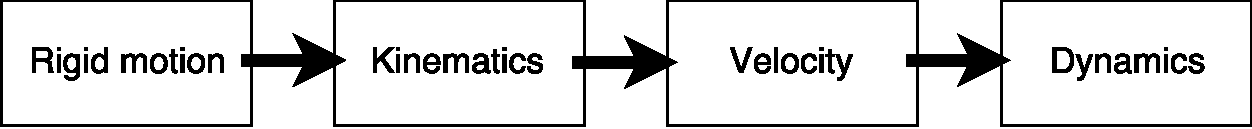
\includegraphics[width=\linewidth]{theory_overview.pdf}
 \caption{Four main parts required to describe the dynamics of a robot}
 \label{theory_overview}
\end{figure}

\section{Rigid motion}
\subsection{Position and rotation}
\subsubsection{Rotations in three dimensions}

If a reference frame $o_0 x_o y_o z_o$ (denoted $O_0$) is rotated in all three dimensions to $O_1$ the \textit{rotation matrix} can be described as the projection of the unit axis in $O_1$ onto $O_0$ as in \eqref{rotmatrix}. This matrix will be used to express point $p^1$ in the reference frame of $O_0$, \eqref{pointrotation}. The same rotation matrix can also be used as an operator to rotate a vector in a fixed reference frame.
\begin{equation}\label{rotmatrix}
R^0_1=\begin{bmatrix}
x_1\cdot x_0 & y_1\cdot x_0 & z_1\cdot x_0\\ 
x_1\cdot y_0 & y_1\cdot y_0 & z_1\cdot y_0\\ 
x_1\cdot z_0 & y_1\cdot z_0 & z_1\cdot z_0
\end{bmatrix}
\end{equation}

\begin{equation}\label{pointrotation}
p^0 = R^0_1p^1
\end{equation}

If $T^0$ is a linear transformation in $O_0$, the same transformation can be expressed in terms if another reference frame $O_1$ as $T^1$ by the help of \eqref{similaritytrans}. This is described as a \textit{similarity transformation} and can be used to express transformation in different reference frames.

\begin{equation}\label{similaritytrans}
T^1 = (R^0_1)^{-1}T^0 R^0_1
\end{equation}

\subsubsection{Composition of rotational transformations}

If $R^0_1$ and $R^1_2$ represents rotational transformations between reference frames \textit{0, 1} and \textit{1, 2}. Then point $p^2$ can be described in terms of $O_0$ as in \eqref{rotationcomposition}. This will be rotation with respect to the \textit{current frame}, which will change as as the transformation happen. If a \textit{fixed axis rotation} is wanted instead, the rotation composition has to be pre multiplied instead of post multiplied, shown in \eqref{rotationcomposition_pre}. As a result it is possible to find a single rotation matrix \textit{$R^i_n$} which describes the combination of an infinite amount of dependent rotations from \textit{i} to \textit{n}, \eqref{Rcompositioninf}.


\begin{equation}\label{rotationcomposition}
p^0 = R^0_1 R^1_2 p^2
\end{equation}

\begin{equation}\label{rotationcomposition_pre}
p^0 = R^1_2 R^0_1 p^2 = R R^0_2 p^2
\end{equation}

\begin{equation}\label{Rcompositioninf}
R^i_n = \prod_{i=0}^{n-1} R^i_{i+1}
\end{equation}


\subsubsection{Parametrisation of rotations}

In equation \eqref{rotmatrix} the transformation were described in terms of nine independent variables. A rotation in 3D can at most have three independent variables and it is therefore convenient to perform a parametrization to get three independent variables. This can be done by using \textit{euler angles}, \textit{roll pitch yaw} or \textit{axis/angle} representation. The euler angle rotation is rotation about ZYZ axis by an amount $\phi, \theta, \psi$ respectively, see \eqref{eulertrans}. \textit{C} and \textit{s} represents the cosine and sine functions respectively. Yaw, Pitch and Roll rotations are rotations around XYZ relative to a fixed frame an described in \eqref{ywapitchroll}.
\begin{align}\label{eulertrans}
\begin{split}
R_{ZYZ} &= R_{z,\phi}R_{y,\theta}R_{z,\psi} \\
&= \begin{bmatrix}
c_\phi c_\theta c_\psi - s_\phi s_\psi & -c_\phi c_\theta s_\psi - s_\phi c_\psi & c_\phi s_\theta\\ 
s_\phi c_\theta c_\psi + c_\phi s_\psi & -s_\phi c_\theta s_\psi + c_\phi c_\psi  & s_\phi s_\theta \\ 
-s_\theta c_\psi & s_\theta s_\psi & c_\theta
\end{bmatrix}
\end{split}
\end{align}


\begin{align}\label{ywapitchroll}
\begin{split}
R_{XYZ} &= R_{z,\phi}R_{y,\theta}R_{x,\psi} \\
&= \begin{bmatrix}
c_\phi c_\theta & - s_\phi c_\psi + c_\phi s_\theta s_\psi & s_\phi s_\psi + c_\phi s_\theta c_\psi \\ 
s_\phi c_\theta & c_\phi c_\psi + s_\phi s_\theta s_\psi  & - c_\phi s_\psi + s_\phi s_\theta c_\psi \\ 
-s_\theta & c_\theta s_\psi & c_\theta c_\psi
\end{bmatrix}
\end{split}
\end{align}

If $R_{k,\theta}$ describes the rotation about a unit vector $k$ with an angle $\theta$ we get what is called an \textit{axis/angle} rotation. If $R$ is the rotation transformation that aligns the z-axis with $k$, \eqref{similaritytrans} can bu used to derive $R_{k,\theta}$ as in \eqref{axisanglerot}.

\begin{equation}\label{axisanglerot}
R_{k,\theta} = R^{-1} R_{z,\theta} R
\end{equation}

\subsection{Rigid motion}

Rigid motion is a combination of rotation and translation. The matrix form is described as a \textit{homogeneous transformation} and is defined as a set of matrices as in \eqref{homeqn}. \textit{R} is the rotation matrix as described before and \textit{d} is the translation vector with respect to a chosen base frame. The same features of composition as described in \eqref{Rcompositioninf} also applies to homogeneous transformation.

\begin{equation}\label{homeqn}
H = \begin{bmatrix}
R_{3x3} & d_{3x1}\\ 
0_{1x3} & 1_{1x1}
\end{bmatrix}=\begin{bmatrix}
r_{11} & r_{12} & r_{13} & d_{1}\\ 
r_{21} & r_{22} & r_{23} & d_{2}\\ 
r_{31} & r_{32} & r_{33} & d_{3}\\ 
0 & 0 & 0 & 1
\end{bmatrix}
\end{equation}


\section{Kinematics}

To describe the dynamics in a serial manipulator or robots in general it's kinematic relationships has to be used. In this section the forward and inverse kinematics will be described shortly and will form the basis for velocity kinematics and dynamics.

\subsection{Denavit-Hartenberg convention}

The homogeneous transformation as described in \eqref{homeqn} is a matrix of six independent variables. But introducing two constraints on how the reference frames are defined with respect to each other the total number of independent variables can be reduced to four. This is the motivation behind the \textit{\gls{DH}} (DH). This convention also provides a common, well known framework for defining robotic systems among engineers.

A DH transformation is defined as a product of four basic transformations, \eqref{DH}. Where $a_i, \alpha_i, d_i $ and $\theta_i$ represents the link length, link twist, link offset and joint angle respectively, for link number \textit{i}. The transformation from the rigid base frame $0$ to the end effector $n$ will then be the product sum of the transformations for each link, \eqref{DHsum}.

\begin{align}\label{DH}
\begin{split}
A_i &= Rot_{z,\theta_i}Trans_{z,d_i}Trans_{x,a_i}Rot_{x,\alpha_i} \\
&= \begin{bmatrix}
c_{\theta_i} & -s_{\theta_i}c_{\alpha_i} & s_{\theta_i}s_{\alpha_i} & a_{i}c_{\theta_i} \\ 
s_{\theta_i} & c_{\theta_i}c_{\alpha_i} & -c_{\theta_i}s_{\alpha_i} & a_{i}s_{\theta_i} \\ 
0 & s_{\alpha_i} & c_{\alpha_i} & d_i \\ 
0 & 0 & 0 & 1 
\end{bmatrix}
\end{split}
\end{align}

\begin{equation}\label{DHsum}
T^0_n=\prod_{i=1}^{n}A_i
\end{equation}

In essence, this establishes the forward kinematic relationship. Each link in the robot can be defined as in \eqref{DH} where either $\theta_i$ or $d_i$ is the varying variable depending on the joint is revolute or prismatic. Lastly, \eqref{DHsum} will give the position and rotation of the end effector with respect to the base frame.

\subsection{Inverse kinematics}

Given a specific \gls{homo} $H$, the problem of inverse kinematics is to solve the forward kinematic equations for it's joint variables such that the transformation matrix of the robot arm equals that of $H$, \eqref{inverse_kin}.

\begin{equation}\label{inverse_kin}
T^0_n = H
\end{equation}

This approach will at most result in twelve nonlinear equations with twelve unknowns and can be very difficult to solve. It is advised to find a geometric solution as this will shorten the computational \todo{insert reference} time. This approach will depend on the actual configuration of the robot and no further theoretical development on a general basis is needed.

\section{Velocity kinematics}
At this point the forward and inverse relationship for the robot has been defined. This section will describe how the velocity of any point on the robot can be defined with respect to the joint variables and it's velocities. This is important for accurate control of the end effector's velocity and when it comes to 
dynamics as we need to know the velocity and acceleration of the mass centres.
\subsection{Jacobian}

A relationship between the joint velocities and the velocity of a specific point on the robot has to be established. This is the purpose of the $Jacobian$ related to that point, \eqref{jacobian}. Where the linear and angular velocity of point $n$ with respect to the base frame $O_0$, $V^0_n$ and $\omega^0_n$ respectively is a product of the Jacobian $J$ and the joint velocities $\dot{q}$. 

\begin{align}\label{jacobian}
\begin{split}
\xi &= J\dot{q}\\
\begin{bmatrix}
V^0_n\\ 
\omega^0_n
\end{bmatrix}_{6\times 1}
&=
\begin{bmatrix}
J_v\\ 
J_\omega
\end{bmatrix}_{6\times n} \begin{bmatrix}
\dot{q}
\end{bmatrix}_{n\times 1}
\end{split}
\end{align}

\begin{equation}\label{Jvel}
J_v = \begin{bmatrix}
J_{v_1} & J_{v_2} & ... & J_{v_n}
\end{bmatrix}
\end{equation}

\begin{equation}\label{Jomega}
J_{\omega} = \begin{bmatrix}
z_0 & z_1 & ... & z_{n-1}
\end{bmatrix}
\end{equation}

\begin{equation}\label{Jvi}
J_{v_i} = z_{i-1}\times (O_n - O_{i-1})
\end{equation}

Each part of the Jacobian, \Crefrange{Jvel}{Jvi} describes how the rotation of one joint affects the velocity at point $n$. The values can be found from the correct columns in the corresponding homogeneous transformation, \eqref{homeqn} describing that point. Specifically, $z=\begin{matrix}[
r_{13} & r_{23} & r_{33}]
\end{matrix}^T$ and $O=\begin{matrix}[
d_{1} & d_{2} & d_{3}]
\end{matrix}^T$.

\eqref{jacobian} provides the linear and angular velocity vectors of the point in question. The absolute velocity can then be calculated by \eqref{absvel}. Here the superscript $0$ are left out for simplicity and $r_n$ denotes the vector from the base frame to the point $n$.

\begin{equation}\label{absvel}
v_{n}=V_n+\omega_n\times r_n
\end{equation}

\subsection{Force and torque relationship}

The Jacobian in \eqref{jacobian} has a special property. If $F = \begin{matrix}[
F_{x} & F_{y} & F_{z} & n_x & n_y & n_z]^T
\end{matrix}$ is the force and torque vector at the end effector, the transpose of the Jacobian then describes the torques at each joint, \eqref{Jtorque}. This will prove helpful when the same equation can be used to find torques at the joints because of dynamic forces.\todo{follow up on this}

\begin{equation}\label{Jtorque}
\tau = J^T F
\end{equation}

\subsection{Inverse velocity and acceleration}
\todo[inline]{
\textbf{Todo}

 - Decide if this section is not needed for my project
}
\section{Dynamics}

\begin{figure}[h!]    
    \centering           
    \def\svgwidth{\columnwidth}
    \input{inkscape/speed.pdf_tex}
    \caption{Velocity and acceleration properties}
    \label{speed}
\end{figure}

\begin{figure}[h!]    
    \centering           
    \def\svgwidth{\columnwidth}
    \input{inkscape/forces.pdf_tex}
    \caption{Forces and torques acting on a robot}
    \label{forces}
\end{figure}

\begin{figure}[h!]    
    \centering           
    \def\svgwidth{\columnwidth}
    \input{inkscape/physical.pdf_tex}
    \caption{Physical dimensions and properties}
    \label{physical}
\end{figure}


\subsection{Euler-Lagrange equations}
\todo[inline]{
\textbf{Todo}

- It seems like this is more on theoretical background on the topic of virtual work, not very relevant when it comes to practical use. Maybe drop this?
}

\subsection{Mass and moment of inertia}
\todo[inline]{
\textbf{Todo}

- explain how the inertia tensor is calculated

- explain how the total mass can be modelled as a single mass point in some cases
}

\subsection{Kinetic and potential energy}

\todo[inline]{
\textbf{Todo}

- Maybye this section is not needed at all
}

Any applied force or torque to a system will result in a change in kinetic and potential energy. It is therefore valuable to describe these relations as this will aid in the process of finding the required torques at each link to achieve a specific movement.

The kinetic energy $K$ of a single body is described in \eqref{kineticE}. Note that the linear and angular velocity, $v$ and $\omega$, are the velocities of the center of mass for that body with respect to the fixed frame. The frame attached to this point is called the \glsf{bodyframe} and are used for most of the calculations when it comes to dynamics. $\mathbf{I}$ represents the inertia tensor with respect to the inertial frame. \todo{describe inertial frame} This tensor will change with the configuration of the body, but the inertia tensor with respect to the \gls{bodyframe} $I$ will stay constant. These are related as in \eqref{Irelated}.

\begin{equation}\label{kineticE}
K = \frac{1}{2}mv^Tv + \frac{1}{2}\omega ^{T}  I \omega
\end{equation}

\begin{equation}\label{Irelated}
\mathbf{I} = RIR^T
\end{equation}

The potential energy is simply the mass times gravity and height, \eqref{potentialE}. $r_c$ is the vector from the reference frame to the mass center.

\begin{equation}\label{potentialE}
P = mg^Tr_c
\end{equation}



\subsection{Newton-Euler formulation}

An interesting and maybe the most important question that can be asked when it comes to dynamics for a robot is the following: What kind of torques on each link $\mathbf{\tau}(t)$ is needed to perform a particular movement $\mathbf{q}(t)$? Or put in another way, given the current position, velocity and acceleration $\mathbf{q}, \mathbf{\dot{q}}$ and $ \mathbf{\ddot{q}}$, what is the resulting torque $\mathbf{\tau}$? One method to solve this is with the \glsf{nef}. This method is especially relevant for computer calculations because of it's recursive nature. With reference to the generalized link $i$ in \figref{newtonEuler}, the  \gls{nef} will now be described in it's two steps, forward and backward recursion.

\begin{figure}[h!]    
    \centering           
    \def\svgwidth{\columnwidth}
    \begin{algorithm}[H]
\DontPrintSemicolon
	\textbf{Forward step}\;
	$\omega_0, \alpha_0, a_{c,0}, a_{e,0} = 0$  \tcp*[f]{joint 0 is always fixed}\;
	 \For{link i=1,2,...,n}{
		  solve $\omega_i$ from (\ref{omega})\;
		  solve $\alpha$ from (\ref{alpha})\;
		  solve $a_{e,i}$ from (\ref{a_end})\;
		  solve $a_{c,i}$ from (\ref{a_center})\;
	 }
	 \BlankLine
	\textbf{Backward step}\;
	$f_{n+1}, \tau_{n+1} = 0$  \tcp*[f]{if no load at end effector}\;
	$f_{n+1}, \tau_{n+1} = f_e, \tau_e$  \tcp*[f]{if load at end effector}\;
	 \For{link i=n,n-1,...,1}{
		  solve $f_i$ from (\ref{linear_equi})\;
		  solve $\tau_i$ from (\ref{angular_equi})\;
	 }
	 
 \caption{Newton-Euler method}\label{nefAlgo}
\end{algorithm}
    \caption{Newton-Euler variables for link i}
    \label{newtonEuler}
\end{figure}

On a general level, \gls{nef} works by setting the change in linear and angular momentum, \eqref{linear_mom} and \eqref{angular_mom} respectively, equal to it's applied forces and torques. The forward step starts with link $1$ and continues until link $n$. Joint zero is always fixed so $\omega_0, \alpha_0, a_{c;0}, a_{e,0}$ are all zero. Then solve $\omega_0, \alpha_0, a_{c;0}, a_{e,0}$ from \Crefrange{omega}{a_center}.

\begin{equation}\label{linear_mom}
\dot{p}_i = m_i a_{ci}
\end{equation}

\begin{equation}\label{angular_mom}
\dot{h}_i = I_i \alpha_i + \omega_i \times \left ( I_i \omega_i \right )
\end{equation}

\begin{align}\label{omega}
\begin{split}
\omega_i &= \left ( R^{i-1}_i \right )^T\omega_{i-1} + b_i\dot{q}_i\\
b_i &= \left ( R^0_i \right )^T z_{i-1}
\end{split}
\end{align}

\begin{equation}\label{alpha}
\alpha_i = \left ( R^{i-1}_i \right )^T\alpha_{i-1} + b_i\ddot{q}_i+\omega_i \times b_i\dot{q}_i
\end{equation}

\begin{equation}\label{a_end}
a_{e,i} = \left ( R^{i-1}_i \right )^T a_{e,i-1} + \dot{\omega}_i \times r_{i,i+1}+\omega_i \times \left ( \omega_i \times r_{i,i+1} \right )
\end{equation}

\begin{equation}\label{a_center}
a_{c,i} = \left ( R^{i-1}_i \right )^T a_{e,i-1} + \dot{\omega}_i \times r_{i,ci}+\omega_i \times \left ( \omega_i \times r_{i,ci} \right )
\end{equation}

Lastly, the backward recursion starts with the last link $n$ and works itself backward until link 1. This step finds the force and torque in each link by solving the equilibrium in \Crefrange{linear_equi}{angular_equi}. An overview of the \gls{nef} as an algorithm is presented in \algref{nefAlgo}.

\begin{equation}\label{linear_equi}
\dot{p}_i = f_i - R^i_{i+1} f_{i+1} + m_i g_i
\end{equation}

\begin{equation}\label{angular_equi}
\dot{h}_i = \tau_i - R^i_{i+1}\tau_{i+1} + f_i \times r_{i,ci}-\left ( R^i_{i+1}f_{i+1} \right ) \times r_{i+1,ci}
\end{equation}

\begin{algorithm}[H]
\DontPrintSemicolon
	\textbf{Forward step}\;
	$\omega_0, \alpha_0, a_{c,0}, a_{e,0} = 0$  \tcp*[f]{joint 0 is always fixed}\;
	 \For{link i=1,2,...,n}{
		  solve $\omega_i$ from (\ref{omega})\;
		  solve $\alpha$ from (\ref{alpha})\;
		  solve $a_{e,i}$ from (\ref{a_end})\;
		  solve $a_{c,i}$ from (\ref{a_center})\;
	 }
	 \BlankLine
	\textbf{Backward step}\;
	$f_{n+1}, \tau_{n+1} = 0$  \tcp*[f]{if no load at end effector}\;
	$f_{n+1}, \tau_{n+1} = f_e, \tau_e$  \tcp*[f]{if load at end effector}\;
	 \For{link i=n,n-1,...,1}{
		  solve $f_i$ from (\ref{linear_equi})\;
		  solve $\tau_i$ from (\ref{angular_equi})\;
	 }
	 
 \caption{Newton-Euler method}\label{nefAlgo}
\end{algorithm}





